\resizebox{\columnwidth}{!}{
    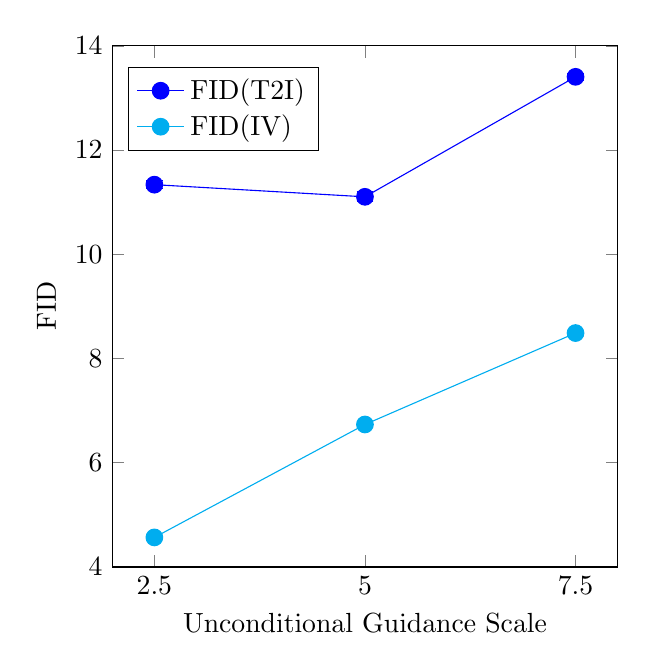
\begin{tikzpicture}
    \begin{axis}[
        xlabel=Unconditional Guidance Scale,
        ylabel=FID,
        xmin=2,
        xmax=8,
        ymin=4,
        ymax=14,
        xtick={2.5,5.0,7.5},
        width=8cm,height=8.2cm,
        legend style={at={(0.22,0.96)},anchor=north,legend cell align=left},
    ]
    \addplot+[
        blue,
        mark=*, mark size=3pt, mark options={fill=blue},
        error bars/.cd,y dir=both,y explicit,
    ] coordinates {
        (2.5, 11.3355988257) +- (0, 0.0796762530121)
        (5.0, 11.1023553055) +- (0, 0.0916626027159)
        (7.5, 13.405008415)  +- (0, 0.0681356441779)
    };\label{t2i-fid}\addlegendentry{FID(T2I)}
    \addplot+[
        cyan,
        mark=*, mark size=3pt, mark options={fill=cyan},
        error bars/.cd,y dir=both,y explicit,
    ] coordinates {
        (2.5, 4.56646982092) +- (0, 0.0211169100996)
        (5.0, 6.7336671616) +- (0, 0.0299270554132)
        (7.5, 8.48817909203)  +- (0, 0.0205315863737)
    };\label{iv-fid}\addlegendentry{FID(IV)}
    \end{axis}
    \end{tikzpicture}
}